% Framework figure v5 (TikZ-native, strict-zone layout).
%
% Layout discipline:
%   Left zone (seller-side)   : x in [  0 mm,  98 mm ]
%   Wall column (firewall)    : x in [ 100 mm, 108 mm ]   <-- only wall + badge
%   Right zone (reviewer-side): x in [ 112 mm, 218 mm ]
%
% Every node is sized so it cannot cross its zone boundary.  The wall is
% a single vertical line at x = 104 mm with the firewall badge centred on
% that line.  Cross-wall arrow has its own dedicated horizontal lane below
% all left-zone content.

\documentclass[tikz,border=4pt]{standalone}

\usepackage{amsmath,amssymb,bm}
\usepackage[T1]{fontenc}
\usepackage[utf8]{inputenc}
\usepackage{newtxtext,newtxmath}
\usepackage{tikz}
\usetikzlibrary{positioning, arrows.meta, calc, shapes.geometric}

% ---- Morandi palette --------------------------------------------------------
\definecolor{mistOne}{HTML}{F3EEE8}
\definecolor{mistTwo}{HTML}{D8D1C7}
\definecolor{mistThree}{HTML}{8A9199}
\definecolor{sageOne}{HTML}{E7E1D6}
\definecolor{sageTwo}{HTML}{B7A99A}
\definecolor{sageThree}{HTML}{5F6E62}
\definecolor{roseOne}{HTML}{F2E9E6}
\definecolor{roseTwo}{HTML}{D8C3BC}
\definecolor{roseThree}{HTML}{9D5454}
\definecolor{ink}{HTML}{1F1F1F}
\definecolor{inkTwo}{HTML}{3D3D3D}
\definecolor{wallDark}{HTML}{2C2A28}
\definecolor{alarm}{HTML}{B14A4A}
\definecolor{pageBg}{HTML}{FAFAF8}

% ---- Reusable node styles ---------------------------------------------------
\tikzset{
  every node/.style = {font=\sffamily\small, align=center},
  % Full-width banners (spans the whole 218 mm canvas).
  bannerR/.style = {draw=roseThree!75!black, fill=roseThree!12,
                     rounded corners=2pt, inner sep=7pt, line width=0.5pt,
                     text width=216mm},
  bannerM/.style = {draw=mistThree!75!black, fill=mistTwo!45,
                     rounded corners=2pt, inner sep=7pt, line width=0.5pt,
                     text width=216mm},
  % Zone titles
  zoneTitleS/.style = {anchor=west, font=\sffamily\bfseries\small\itshape,
                       color=sageThree, inner sep=0pt},
  zoneTitleR/.style = {anchor=west, font=\sffamily\bfseries\small\itshape,
                       color=mistThree!70!black, inner sep=0pt},
  % Left-zone boxes (max ~98mm wide effectively).
  imgBox/.style   = {draw=sageThree, fill=white, rounded corners=3pt,
                     inner sep=4pt, line width=0.9pt, minimum height=11mm,
                     text width=24mm, font=\sffamily\small},
  pipeBox/.style  = {draw=sageThree, fill=sageOne, rounded corners=3pt,
                     inner sep=3pt, line width=0.6pt, minimum height=11mm,
                     text width=28mm, font=\sffamily\small},
  etBox/.style    = {draw=sageThree, fill=sageTwo!70, rounded corners=3pt,
                     inner sep=3pt, line width=0.6pt, minimum height=11mm,
                     text width=8mm,  font=\sffamily\bfseries},
  vAncBox/.style  = {draw=sageThree, fill=sageThree, rounded corners=3pt,
                     inner sep=3pt, line width=0.6pt, minimum height=11mm,
                     text width=16mm, text=white,
                     font=\sffamily\bfseries\small},
  rowBox/.style   = {draw=inkTwo!85, fill=#1, rounded corners=3pt,
                     inner sep=4pt, line width=0.4pt, minimum height=8mm,
                     text width=92mm, font=\sffamily\small},
  advBox/.style   = {draw=roseThree, fill=roseOne, rounded corners=3pt,
                     inner sep=4pt, line width=0.9pt, minimum height=11mm,
                     text width=64mm, font=\sffamily\small},
  % Right-zone boxes
  queryBox/.style = {draw=mistThree!90!black, fill=white, rounded corners=3pt,
                     inner sep=4pt, line width=0.9pt, minimum height=11mm,
                     text width=58mm, font=\sffamily\small},
  etBoxR/.style   = {draw=mistThree!90!black, fill=mistTwo!75, rounded corners=3pt,
                     inner sep=3pt, line width=0.6pt, minimum height=11mm,
                     text width=8mm,  font=\sffamily\bfseries},
  evalBox/.style  = {draw=mistThree!90!black, fill=mistOne, rounded corners=3pt,
                     inner sep=4pt, line width=0.6pt, minimum height=11mm,
                     text width=98mm, font=\sffamily\small},
  % Firewall badge (centred on the wall line)
  wallLabel/.style = {fill=wallDark, text=white, rounded corners=2pt,
                     inner sep=5pt, font=\sffamily\bfseries\footnotesize,
                     text width=14mm, align=center},
  % Arrows
  flowS/.style    = {-{Stealth[length=2.4mm,width=2mm]},
                     line width=0.7pt, color=sageThree},
  flowR/.style    = {-{Stealth[length=2.4mm,width=2mm]},
                     line width=0.7pt, color=mistThree!75!black},
  flowRose/.style = {-{Stealth[length=2.6mm,width=2.2mm]},
                     line width=1.0pt, color=roseThree},
  wallLine/.style = {line width=0.9mm, color=wallDark},
}

\begin{document}
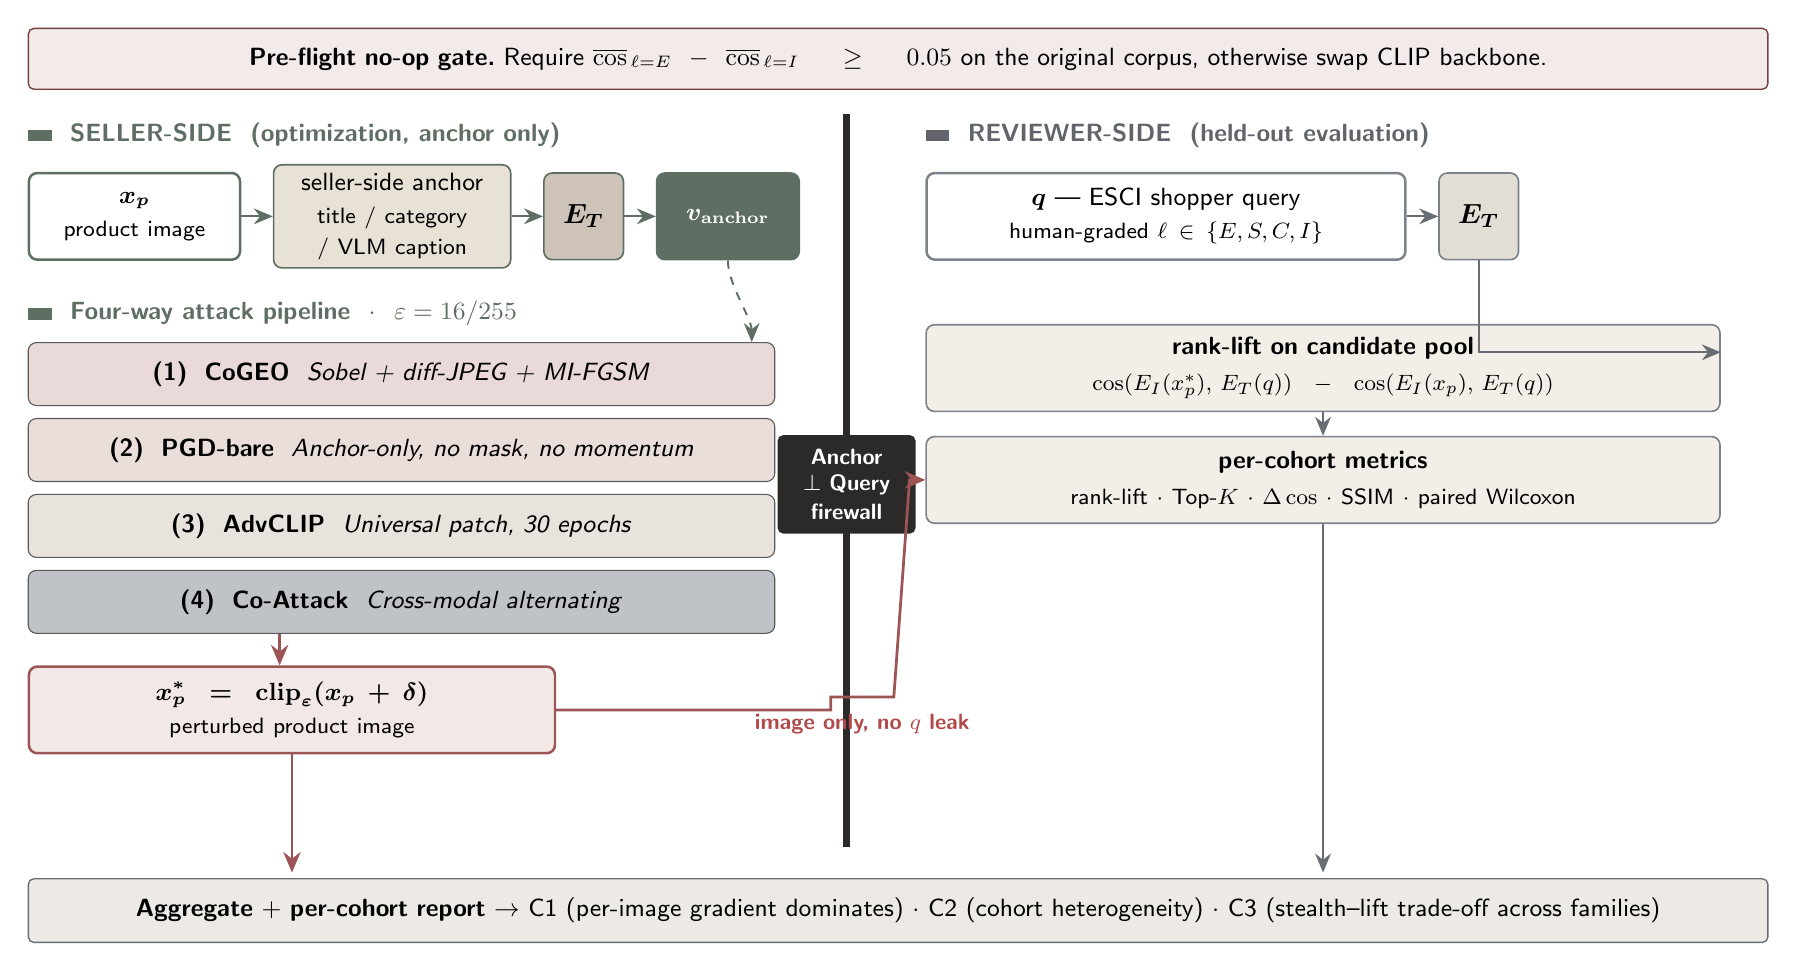
\begin{tikzpicture}[node distance=4mm and 4mm]

% --- Pre-flight banner -------------------------------------------------------
\node[bannerR, anchor=north west] (preflight) at (0mm, 0mm) {%
  \textbf{Pre-flight no-op gate.}\ %
  Require $\overline{\cos}_{\,\ell=E} - \overline{\cos}_{\,\ell=I}\ \geq\ 0.05$
  on the original corpus, otherwise swap CLIP backbone.};

% ============================================================================
% LEFT ZONE: seller-side (anchor only)
% ============================================================================

\node[zoneTitleS, anchor=north west]
  (sellerTitle) at (0mm, -12mm)
  {\textcolor{sageThree}{\rule{3mm}{1.5mm}}\ \ %
   SELLER-SIDE\ \ (optimization, anchor only)};

% Seller pipeline (xp -> anchor -> E_T -> v_anchor) - all left of wall.
\node[imgBox, anchor=north west] (xp)
  at ($(sellerTitle.south west) + (0mm, -3mm)$)
  {$\boldsymbol{x_p}$\\[1pt]\footnotesize product image};
\node[pipeBox, right=of xp]      (anchorBox)
  {seller-side anchor\\[1pt]\footnotesize title / category / VLM caption};
\node[etBox,   right=of anchorBox] (et1) {$\boldsymbol{E_T}$};
\node[vAncBox, right=of et1]       (vanc) {$\boldsymbol{v_{\mathrm{anchor}}}$};

\draw[flowS] (xp.east)        -- (anchorBox.west);
\draw[flowS] (anchorBox.east) -- (et1.west);
\draw[flowS] (et1.east)       -- (vanc.west);

% Four-way attack title and rows (still left zone).
\node[zoneTitleS, anchor=north west]
  (attackTitle) at ($(xp.south west) + (0mm,-5mm)$)
  {\textcolor{sageThree}{\rule{3mm}{1.5mm}}\ \ %
   \textbf{Four-way attack pipeline}\ \ $\cdot$\ \ $\varepsilon = 16/255$};

\node[rowBox=roseThree!22, anchor=north west]
  (m1) at ($(attackTitle.south west) + (0mm,-2mm)$)
  {\textbf{(1)\ \ CoGEO}\ \ \emph{Sobel + diff-JPEG + MI-FGSM}};
\node[rowBox=roseTwo!55, below=1.5mm of m1] (m2)
  {\textbf{(2)\ \ PGD-bare}\ \ \emph{Anchor-only, no mask, no momentum}};
\node[rowBox=mistTwo!60, below=1.5mm of m2] (m3)
  {\textbf{(3)\ \ AdvCLIP}\ \ \emph{Universal patch, 30 epochs}};
\node[rowBox=mistThree!55, below=1.5mm of m3] (m4)
  {\textbf{(4)\ \ Co-Attack}\ \ \emph{Cross-modal alternating}};

% v_anchor feeds attack rows.  Both endpoints are left of the wall, so the
% dashed arrow stays in the left zone.
\draw[flowS, dashed]
  (vanc.south) .. controls +(0,-3mm) and +(0,3mm) ..
  ($(m1.north east) + (-3mm,0)$);

% Perturbed image x_p* (still left zone, directly below the rows).
\node[advBox, anchor=north west]
  (xpstar) at ($(m4.south west) + (0mm,-4mm)$)
  {$\boldsymbol{x_p^* = \mathrm{clip}_{\varepsilon}(x_p + \delta)}$\\[1pt]%
   \footnotesize perturbed product image};
\draw[flowRose] ($(m4.south west) + (32mm, 0)$) -- ($(xpstar.north west) + (32mm,0)$);

% ============================================================================
% WALL: a single vertical line at x = 104 mm with firewall badge.
% ============================================================================

% wallTop is just below preflight; wallBottom is just above claims.
\coordinate (wallTop)    at (104mm, -11mm);
\coordinate (wallBottom) at (104mm, -104mm);

\draw[wallLine] (wallTop) -- (wallBottom);

% Firewall badge: place at vertical mid-point of the wall.
\node[wallLabel] (firewall) at (104mm, -58mm)
  {Anchor $\perp$ Query\\[1pt] firewall};

% ============================================================================
% RIGHT ZONE: reviewer-side (held-out evaluation)
% ============================================================================

\node[zoneTitleR, anchor=north west]
  (reviewerTitle) at (114mm, -12mm)
  {\textcolor{mistThree!70!black}{\rule{3mm}{1.5mm}}\ \ %
   REVIEWER-SIDE\ \ (held-out evaluation)};

\node[queryBox, anchor=north west]
  (q) at ($(reviewerTitle.south west) + (0mm,-3mm)$)
  {$\boldsymbol{q}$\ — ESCI shopper query\\[1pt]\footnotesize%
   human-graded $\ell\!\in\!\{E,S,C,I\}$};
\node[etBoxR, right=of q] (et2) {$\boldsymbol{E_T}$};
\draw[flowR] (q.east) -- (et2.west);

\node[evalBox, anchor=north west]
  (ranklift) at ($(q.south west) + (0mm,-8mm)$)
  {\textbf{rank-lift on candidate pool}\\[2pt]\footnotesize%
   $\cos(E_I(x_p^*),\, E_T(q))\ -\ \cos(E_I(x_p),\, E_T(q))$};
\draw[flowR] (et2.south) |- ($(ranklift.east) + (0, 2mm)$);

\node[evalBox, anchor=north west]
  (cohort) at ($(ranklift.south west) + (0mm,-3mm)$)
  {\textbf{per-cohort metrics}\\[2pt]\footnotesize%
   rank-lift $\cdot$ Top-$K$ $\cdot$ $\Delta\cos$ $\cdot$ SSIM $\cdot$ paired Wilcoxon};
\draw[flowR] (ranklift.south) -- (cohort.north);

% ============================================================================
% CROSS-WALL ARROW: x_p* (image only, no q leak) -> per-cohort metrics.
% Dedicated horizontal lane below the bottom of xpstar.
% ============================================================================

\coordinate (xLeft)  at ($(xpstar.east)  + (2mm, 0mm)$);
\coordinate (xMid)   at (102mm, -85mm);                  % horizontal lane y
\coordinate (xRight) at ($(cohort.west) + (-2mm, 0mm)$);

% Route: xpstar.east -> down to lane y -> across through wall -> up to cohort.west
\draw[flowRose]
  (xpstar.east) -| (102mm, -85mm)
  -- (110mm, -85mm)
  -- ($(cohort.west) + (-2mm, 0mm)$)
  -- (cohort.west);

% "image only, no q leak" annotation, placed under the wall-crossing point.
\node[font=\sffamily\bfseries\footnotesize\itshape, color=alarm,
      anchor=north]
  at (106mm, -86mm)
  {image only, no $q$ leak};

% ============================================================================
% BOTTOM BANNER: claims
% ============================================================================

\node[bannerM, anchor=north west]
  (claims) at (0mm, -108mm)
  {\textbf{Aggregate $+$ per-cohort report}\ $\rightarrow$\ %
   C1 (per-image gradient dominates)\ $\cdot$\ %
   C2 (cohort heterogeneity)\ $\cdot$\ %
   C3 (stealth--lift trade-off across families)};

% Feed arrows down into claims banner from left and right zones
\draw[flowRose]
  (xpstar.south) -- ($(xpstar.south) + (0,-3mm)$)
  -- ($(xpstar.south |- claims.north) + (0,2pt)$);
\draw[flowR]
  (cohort.south) -- ($(cohort.south) + (0,-3mm)$)
  -- ($(cohort.south |- claims.north) + (0,2pt)$);

\end{tikzpicture}
\end{document}
